\subsection{Tracking}

A charged particle produced in a decay of a heavy flavour meson exiting the \pv is first detected
as \emph{hits} in the \velo.
The \velo module is made up of 21 modules orientated in the $x-y$ plane, and
each module consists of two layers of silicon strip detectors with $(r,\phi)$ coordinates.
The pitch of the silicon strips vary from $\sim40\mum$ nearest the centre, where detector occupancy
is highest, to $\sim100\mum$ at the extremities.

Spacial resolution is vitally important so close to the interaction point.
The \velo must be able to resolve all tracks and distinguish \pv{s} coming from
proton-proton interactions, and secondary vertices indicative of decaying heavy flavour hadrons.
For example, a \Bp meson with a momentum of $100\gev$ will travel approximately $1\cm$ before decaying.
This must all be done in a high track multiplicity environment.

%Tracking begins with the \velo which precisely measures spatial
%coordinates of charged particle close to the interaction point.

% increase spatial resolution of vertices,
To decrease the distance of extrapolation of tracks to vertices,
the active area of the \velo starts $8\mm$ from the beam line.
This is made possible because each module is split into two halves which retract when the \lhc beam
is unstable.
Its design leads to a detector with high impact parameter resolution, which can detect tracks
emerging from a proton-proton interaction in the range $1.6<\eta<4.9$ and $|z|<10.6\cm$.
Figure~\ref{fig:lhcb:velo} shows the geometry of the \velo.

\begin{figure}
  \begin{center}
    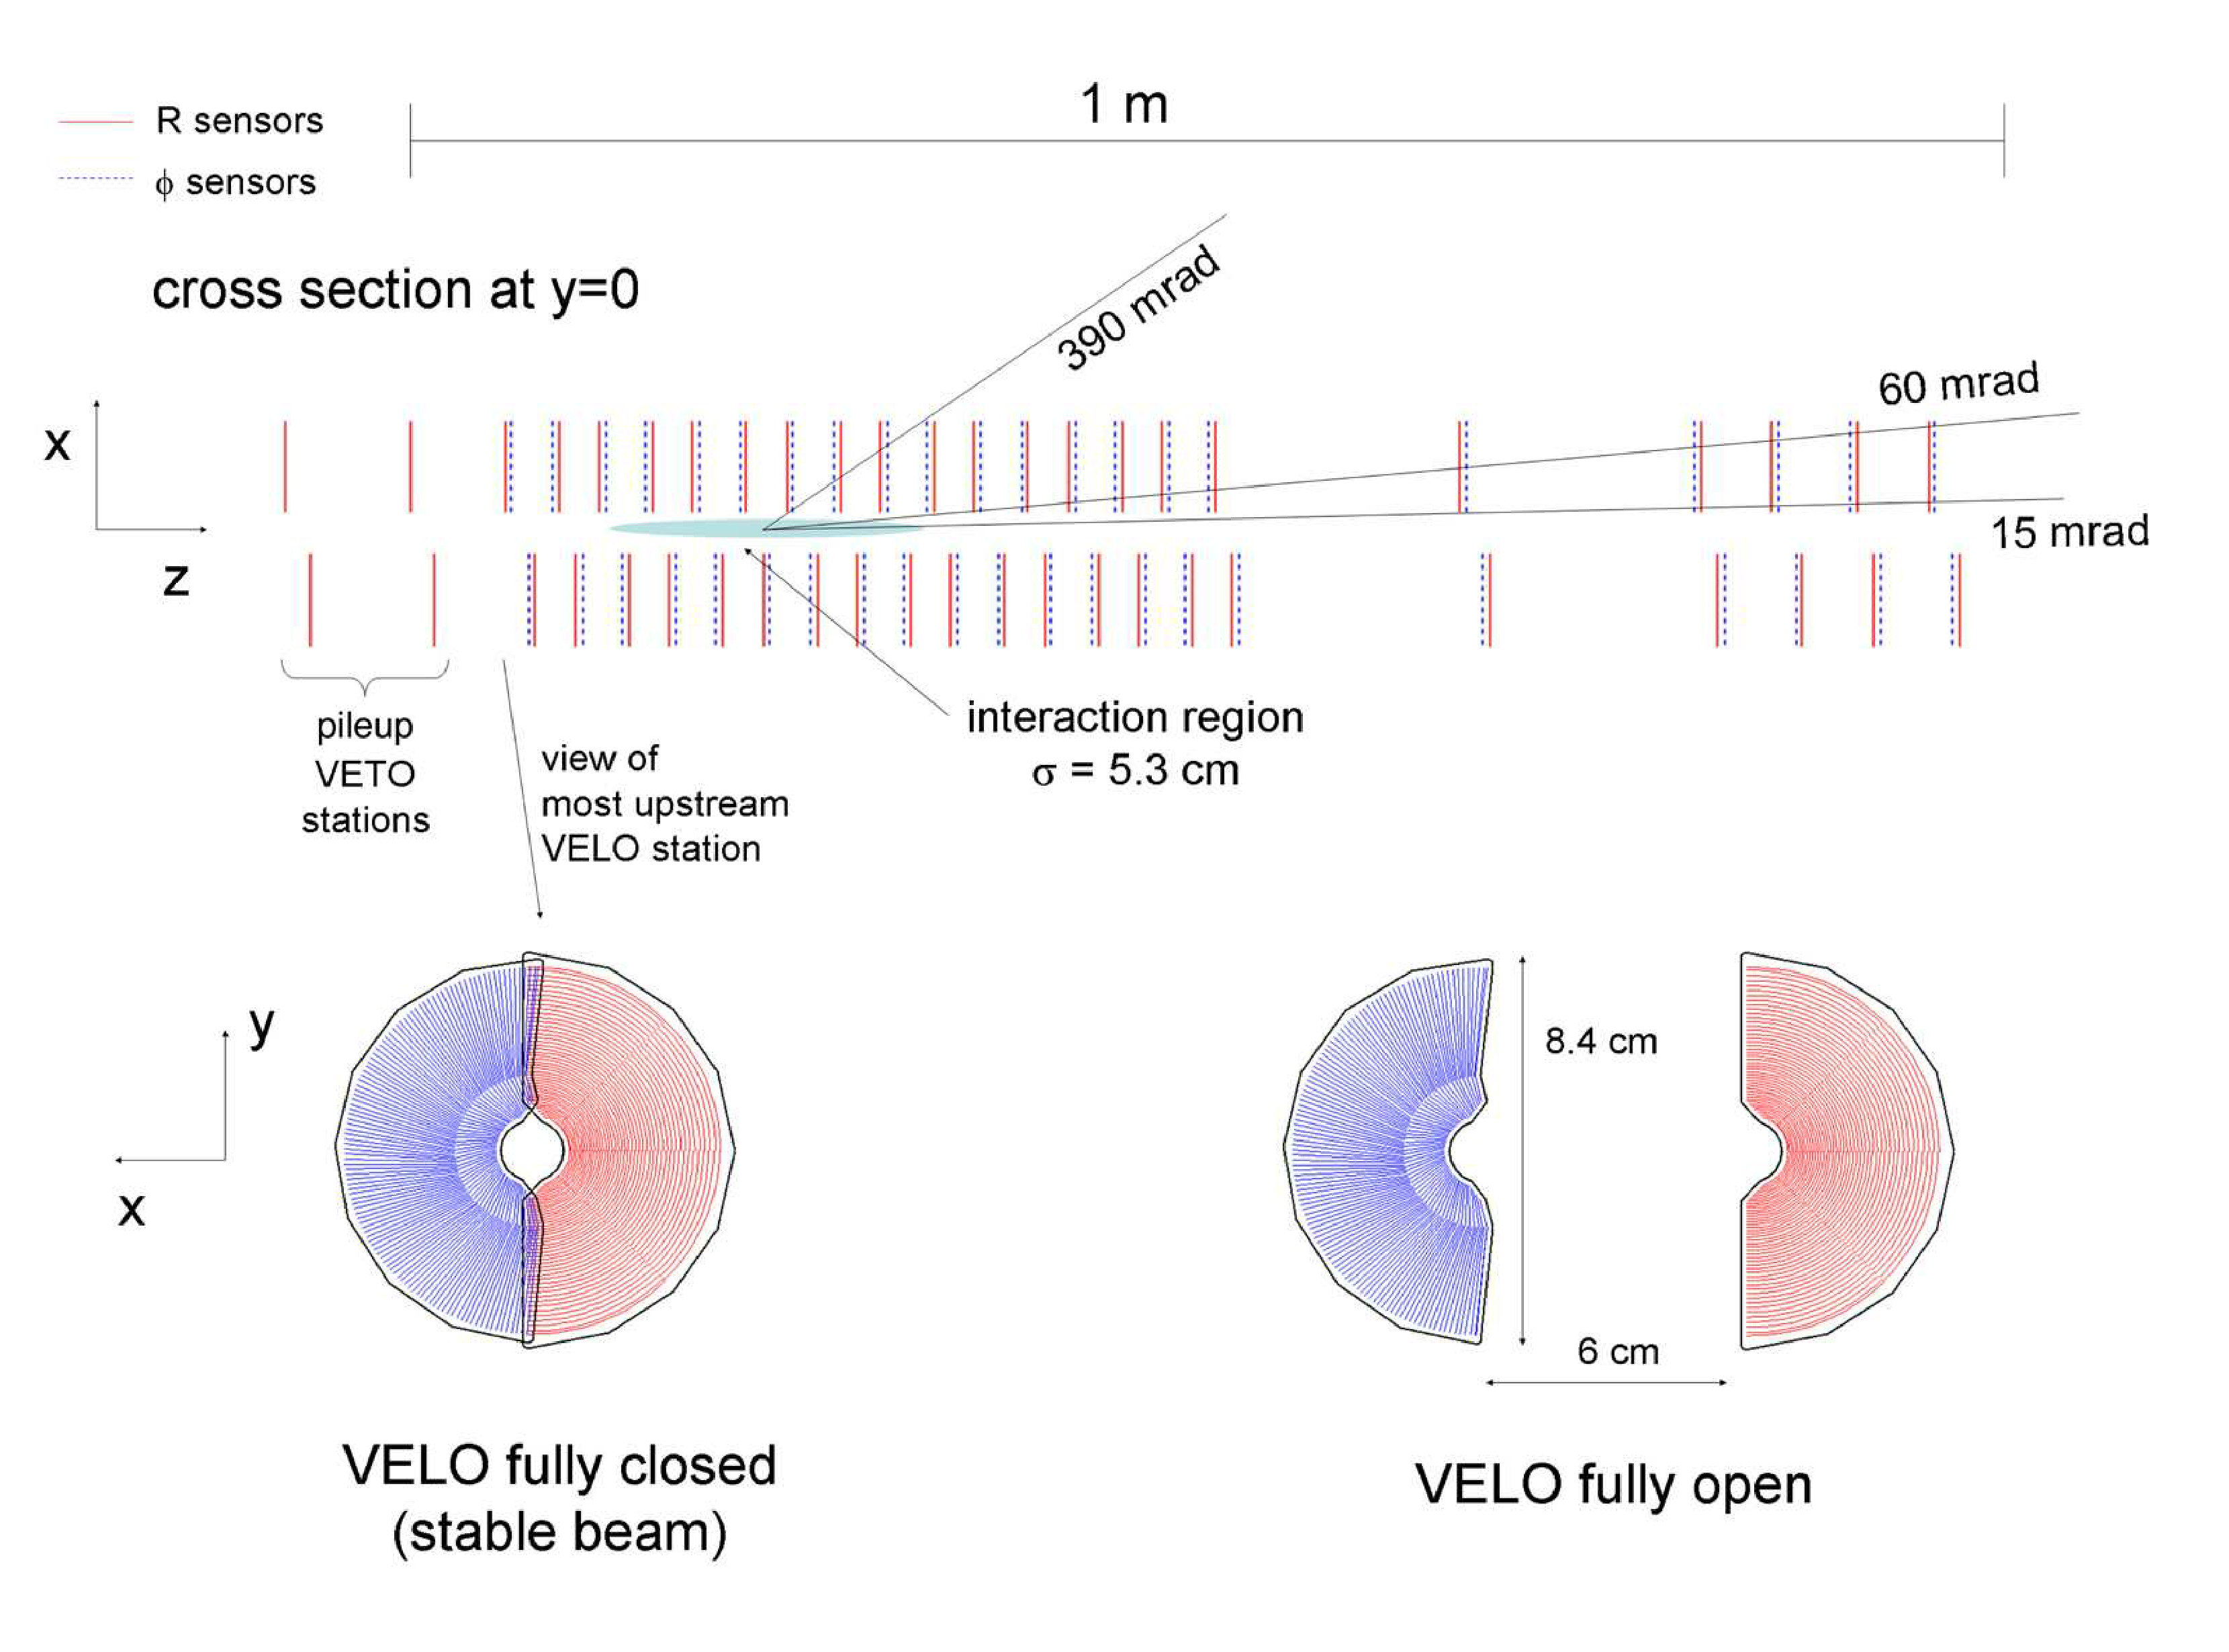
\includegraphics[width=0.7\textwidth]{velo}
  \end{center}
  \caption[LHCb Vertex Locator]
  {\small
    The layout of silicon sensors the \velo in showing $r$ sensors in red and $\phi$ sensors in
    blue.
    A cross section at $y=0$ in the $x-z$ plane is shown while the \velo is closed.
    Along side these are slices in the $x-y$ plane, with the \velo closed and open.
  }
  \label{fig:lhcb:velo}
\end{figure}

Hits recorded in the tracking system are fitted to tracks, and in order to decrease the
distance of extrapolation of tracks to vertices,
the active area of the \velo starts $8\mm$ from the beam line.
This is made possible because each module is split into two halves which are retracted when the
\lhc beam is being injected, and then closed when the beam is declared stable and data taking can
begin.
Its design leads to a detector with high impact parameter resolution, which can detect tracks
emerging from a proton-proton interaction in the range $1.6<\eta<4.9$ and $|z|<10.6\cm$.
The geometry of the tracking stations is shown in \Fig{fig:lhcb:tracking}.

\begin{figure}
  \begin{center}
    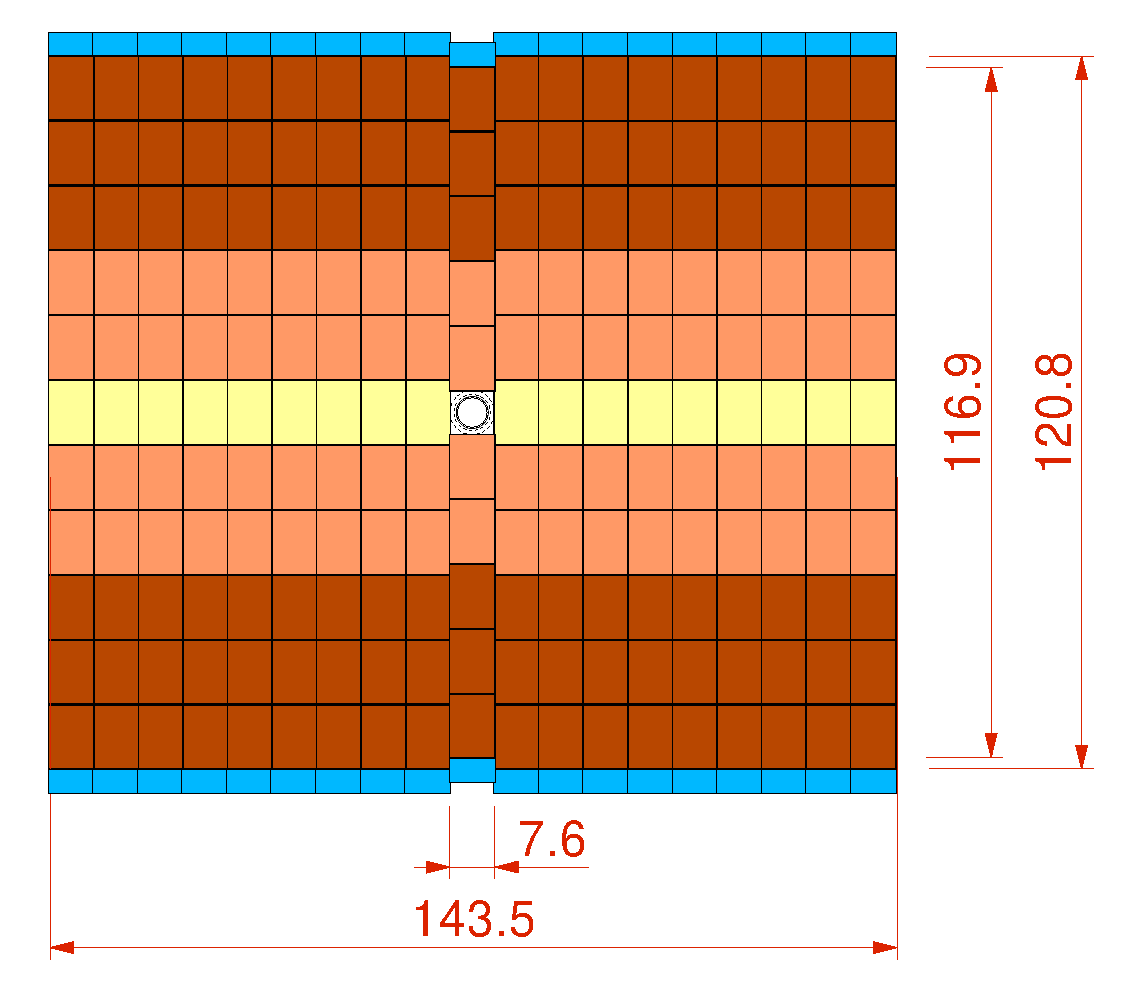
\includegraphics[width=0.5\textwidth]{TTfront}
    \caption[\lhcb TT]
    {\small
      Schematic diagram of a single stereo \ttracker layer oriented in the $x$-direction.
      Different colours indicate readout density.
      All units are in cm.
    }
    \label{fig:lhcb:tt}
  \end{center}
\end{figure}

Charged particles leaving the \velo are next observed traversing the \ttracker (assuming that they
remain within the \lhcb detector volume).
Immediately downstream of the \ttracker is the \lhcb magnet, followed by the remaining three
tracking stations (T1--3).
The T1--3 tracking stations are each made of two different technologies, the area nearest the beam,
aptly named the Inner Tracker (\intr), shares silicon sensor technology adopted by the \ttracker,
while the Outer Tracker (\ot) is uses a straw drift-tube technology.
Each tracking station exhibits an $x-u-v-x$ geometry, where $u$ and $v$ are rotated by $-5^\circ$ and
$+5^\circ$ with respect to the $y$-axis.

Together, the \ttracker and \intr are referred to as the \st.
The \st uses silicon strip sensors with a pitch of $200\mum$.
The \ttracker is the only part of the tracking system that is not used in the trigger, but is
instead used to improve the resolution in reconstructing tracks offline.
To do this, the \ttracker aids the extrapolation of tracks from T1--3, --- and the muon stations
--- to the \velo.
Spacial resolution of the \ttracker is increased by having a large gap, around $27\cm$, between
each stereo layer of the detector, whereas in the \intr the gap is about $4\cm$.
To cope with higher occupancy nearest the beam line, the \ttracker has a increased readout density
closer to $y=0$.
A schematic diagram of a \ttracker layer is shown in \Fig{fig:lhcb:tt}.

Figure~\ref{fig:lhcb:tracking} shows a diagram of T1--3.
The \intr{s} each occupy a small cross-shaped region, is closest to the beam in T1--3.
The \ot is constructed from modules each containing two staggered planes of densely packed straw
tubes, each with a diameter of  $4.9\mm$.
In all the \velo, \st and \ot give the \lhcb detector excellent momentum resolution;
$\tfrac{\Delta p}{p}$ between 0.4 and 0.6\,\% for particles with momenta of $5\gev$ and $100\gev$
respectively.
%Essential for good resolution of the B invariant mass.

\begin{figure}
  \begin{center}
    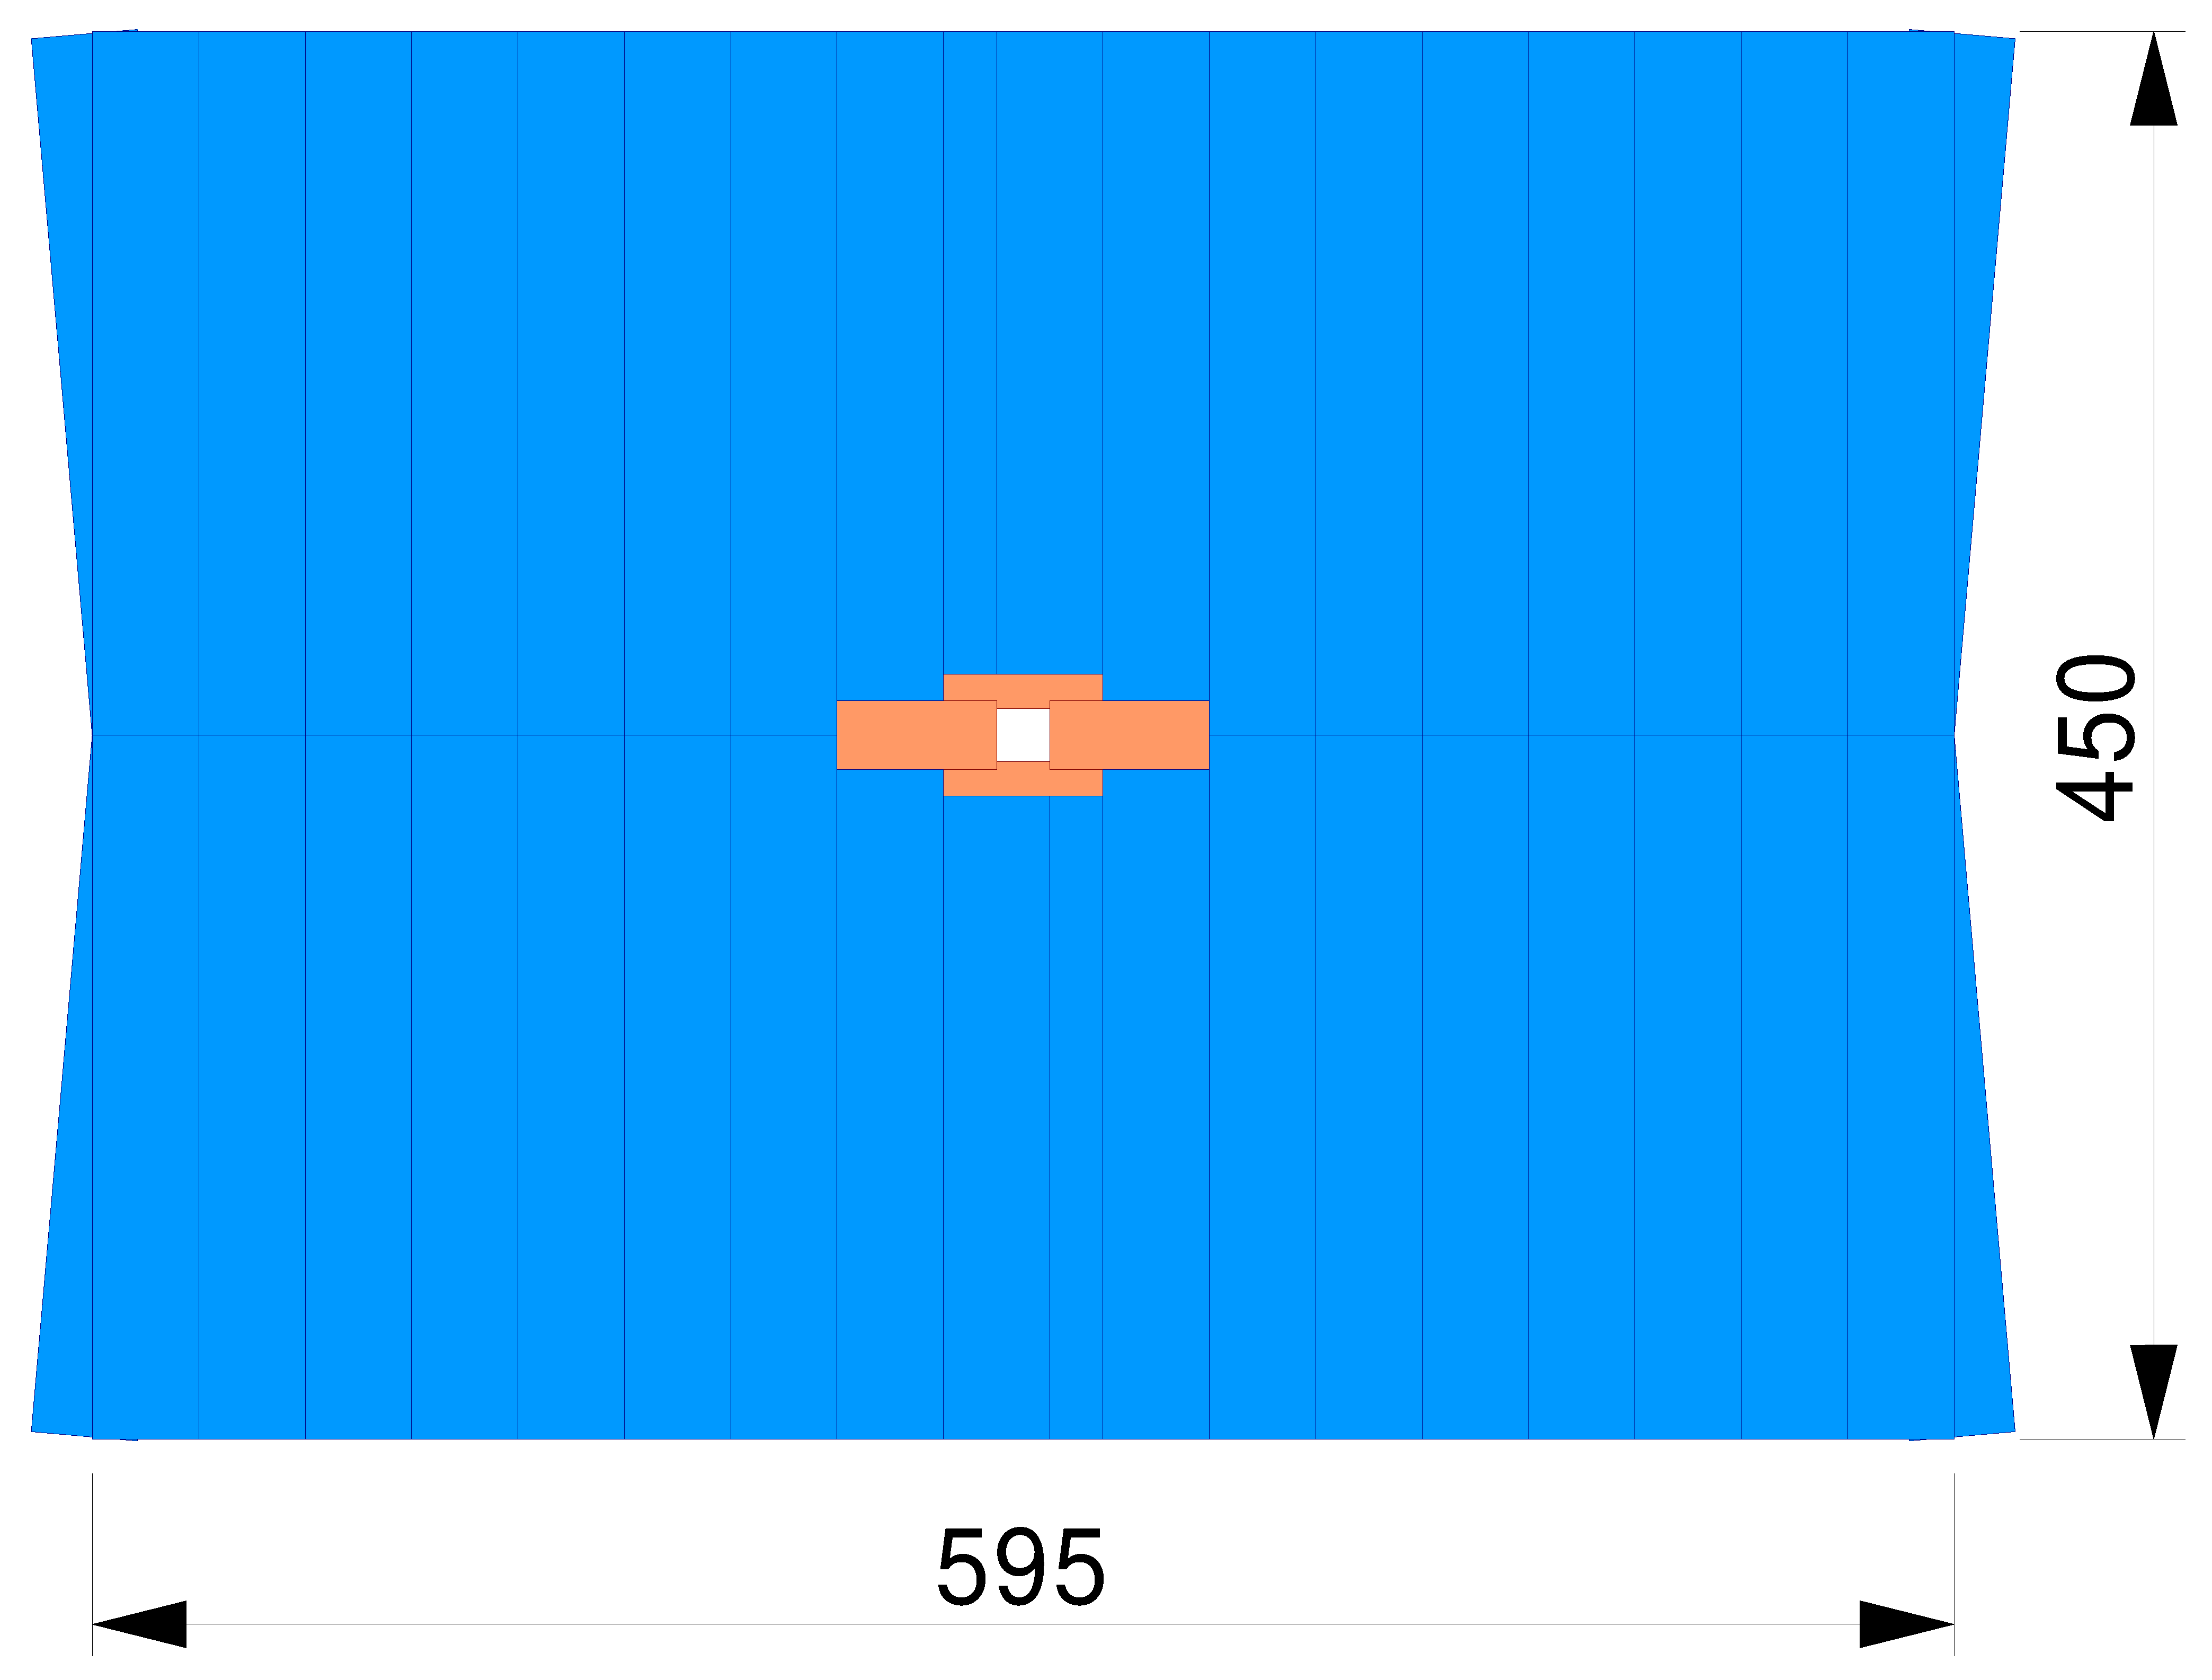
\includegraphics[height=0.18\textheight]{stfront}
    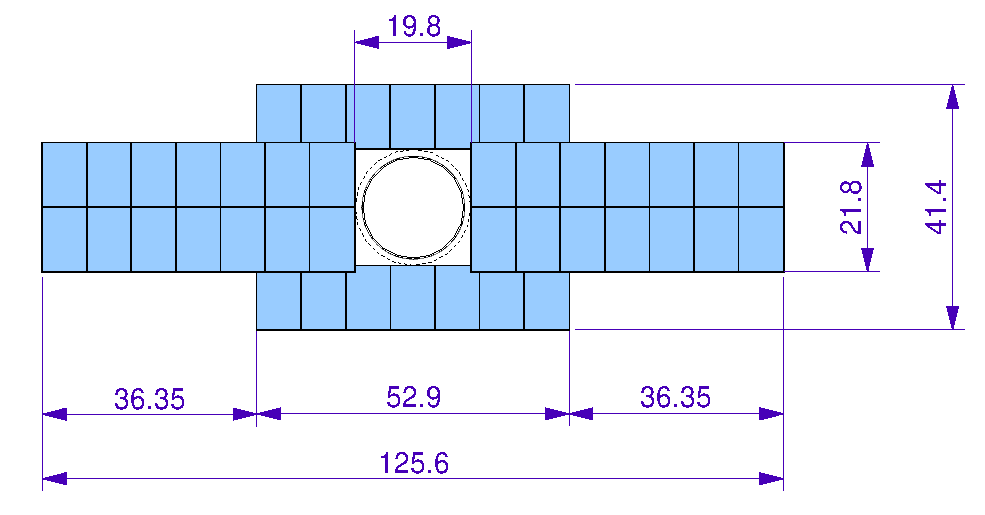
\includegraphics[height=0.19\textheight]{st2}
  \end{center}
  \caption[\lhcb tracking stations]
  {\small
      Schematic diagram of the (left) tracking stations T1--3, where the outer region is the OT,
      and the inner cross is the silicon IT.
      A zoom of an $x$ oriented IT layer is also shown (right).
      All units are in cm.
  }
  \label{fig:lhcb:tracking}
\end{figure}


%\subsection{Particle identification}
%Beauty flavoured hadrons can decay into any (allowed) combination of hadrons and
%leptons.
%Misidentifying daughter particles when reconstructing a candidate $B$ hadron gives rise to a
%combinatorial background making the signal less significant.
%\lhcb can distinguish hadrons from one another using two \rich detectors, and penetrating muons are
%identified by the muon system.


%The \rich detectors work by focusing the Cherenkov light emitted by particles passing through
%given materials, or radiators, onto photomultipliers using spherical mirrors.
%The opening angle of the Cherenkov radiation cone, $\theta_\mathrm{Ch}$ is related to the
%particle's phase velocity, $v_p$, via:
%\begin{align}
  %%\cos\theta_\mathrm{Ch}=\frac1{n\beta}. %, \beta=\frac{v_p}{c}.
  %\cos\theta_\mathrm{Ch}=\frac1{n\beta}, && \beta=\frac{v_p}{c}.
%\end{align}
%With a measurement of the particle's momentum from the tracking system and only a few possible
%masses (that of the electron, muon, pion, kaon or proton) likelihoods are constructed for each
%track based on the ring of photons which such a particle would emit.
%The measured quantity is that of the delta log-likelihood ($\Delta LL(X-\pi$), which is the difference between the
%logarithm of the likelihood of the hypothesis of the particle $X$ compared to the null hypothesis of the
%pion.

%The two \rich detectors at \lhcb contain three different radiators (Aerogel and \cfourften in
%\richone, and \cffour in \richtwo) allowing them to cover different momentum ranges.
%\richone is situated immediately downstream of the \velo and covers the low momentum range,
%$2<p<40\gev$, while \richtwo lies downstream of T3 and covers the range $15<p<100\gev$.
%The variation of $\theta_\mathrm{Ch}$ on momentum for pions, kaons and protons is shown in
%Fig.~\ref{fig:lhcb:pideff}.

%In this way, the \lhcb detector can achieve excellent pion-kaon separation, for a kaon with
%momentum around $20\gev$ the identification rate is near $100\,\%$ and the pion misidentification
%rate is a few percent as shown in Fig.~\ref{fig:lhcb:pideff}.
%%This figure also shows the variation of $\theta_\mathrm{Ch}$ with momentum for pions,
%%kaons and protons; it also shows \lhcb's ability to discriminate between pions and kaons.

%\begin{figure}
  %\begin{center}
    %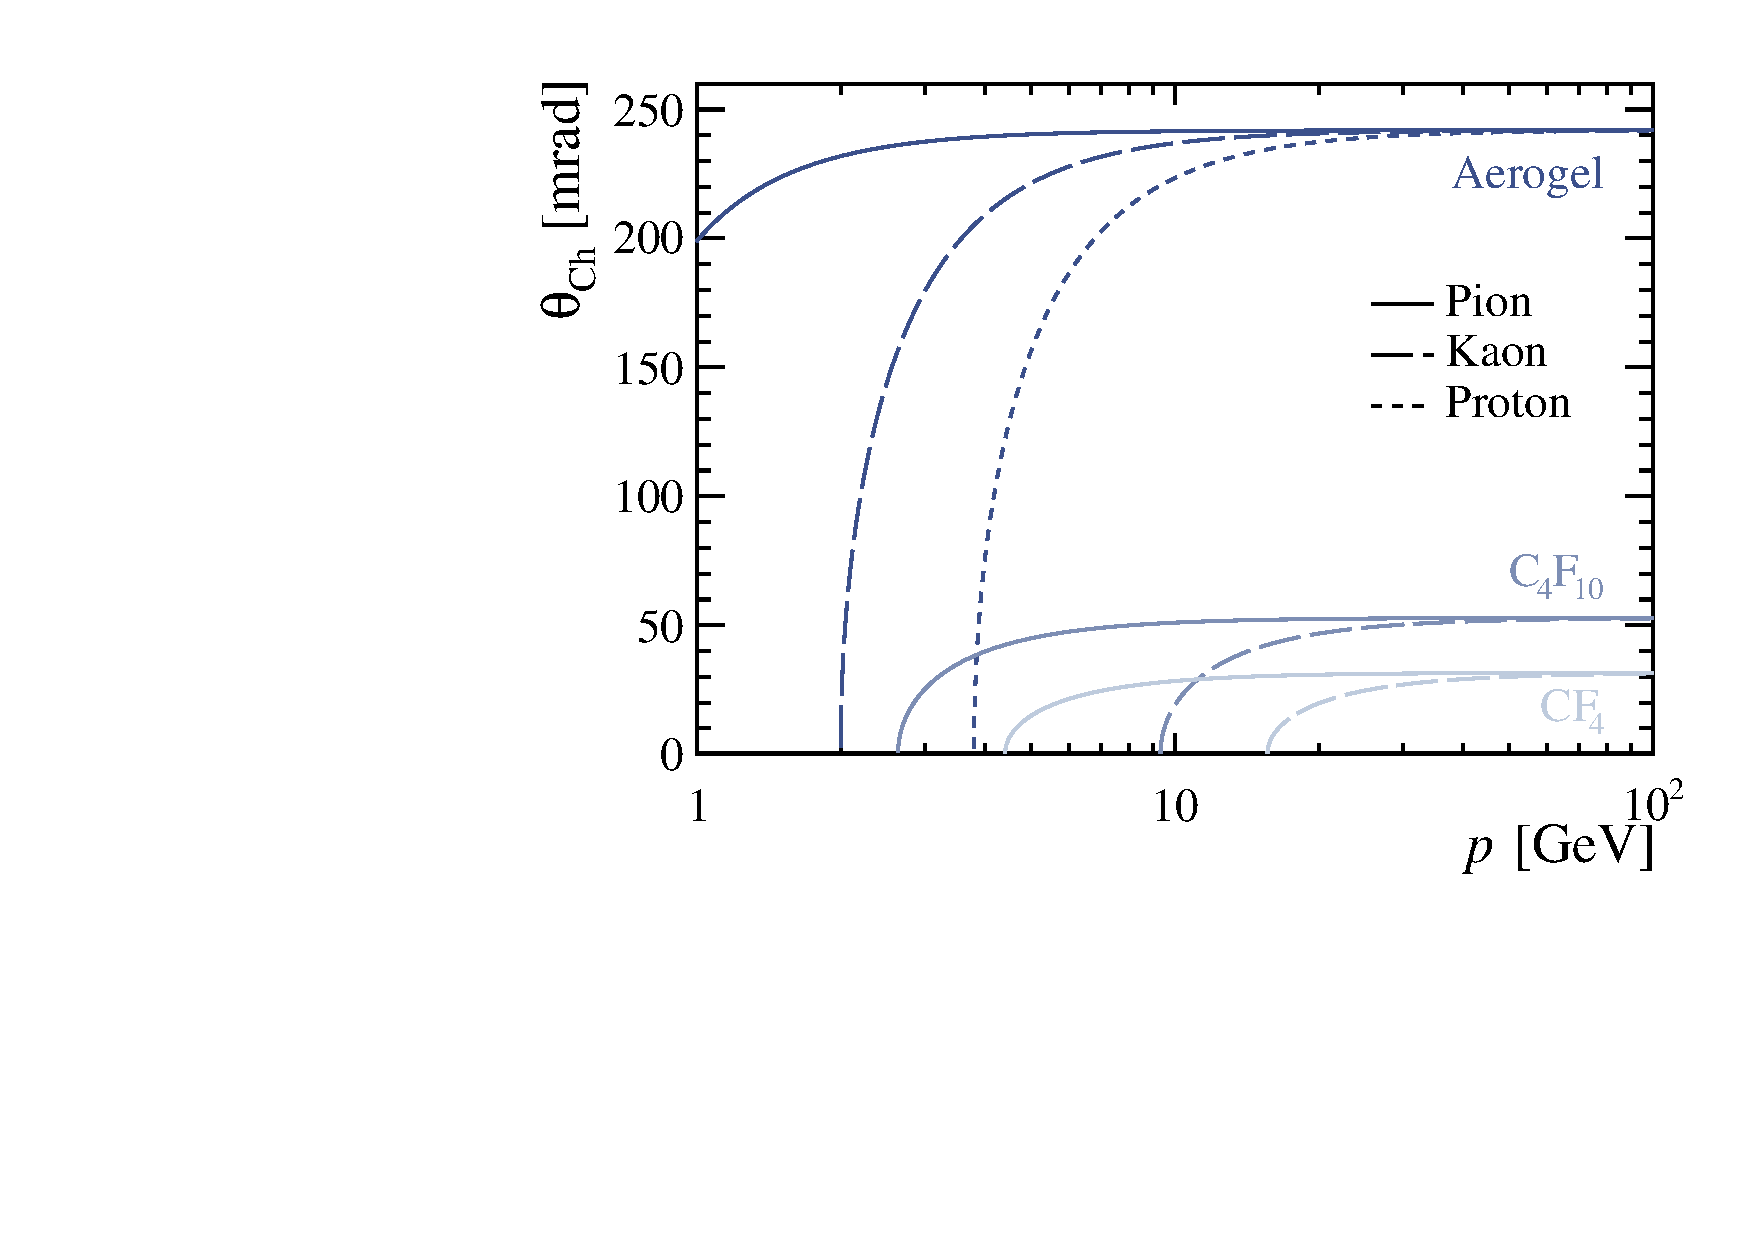
\includegraphics[height=0.2\textheight]{cherenkov_theory}
    %%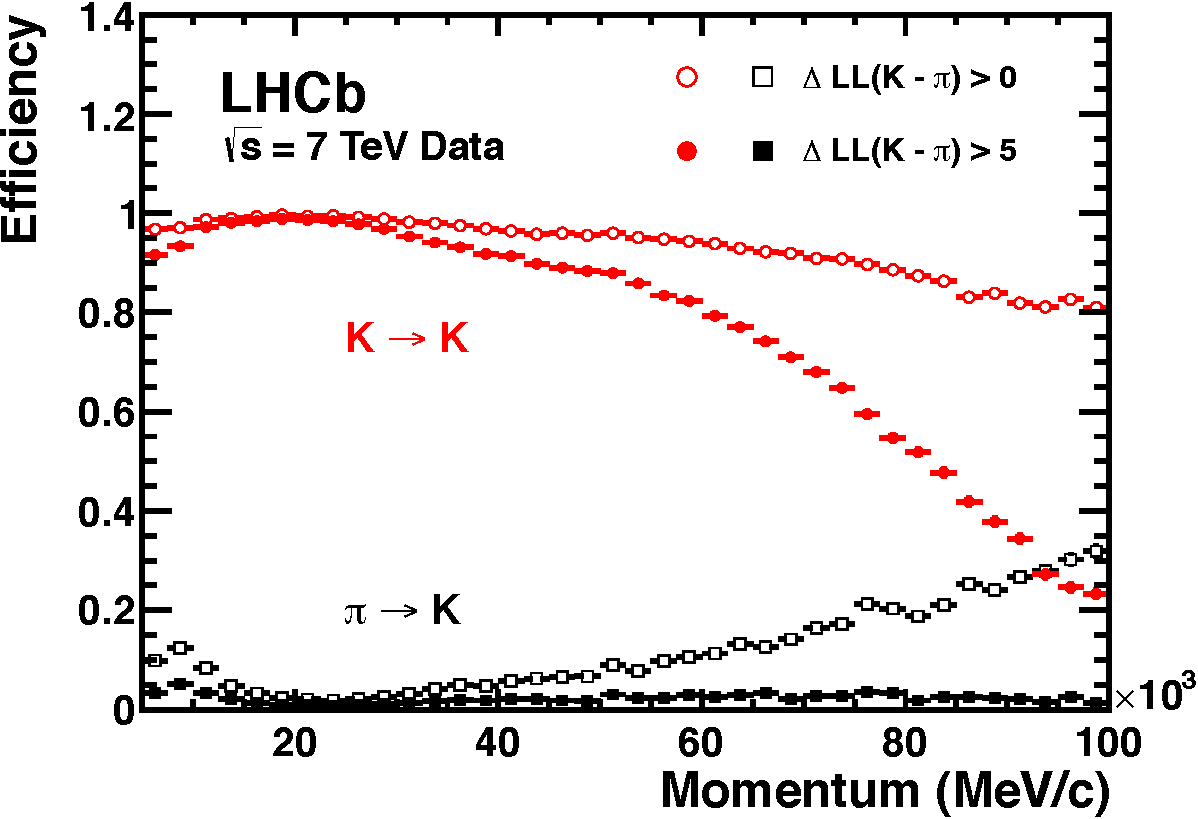
\includegraphics[height=0.2\textheight]{KandPi_2_K}
    %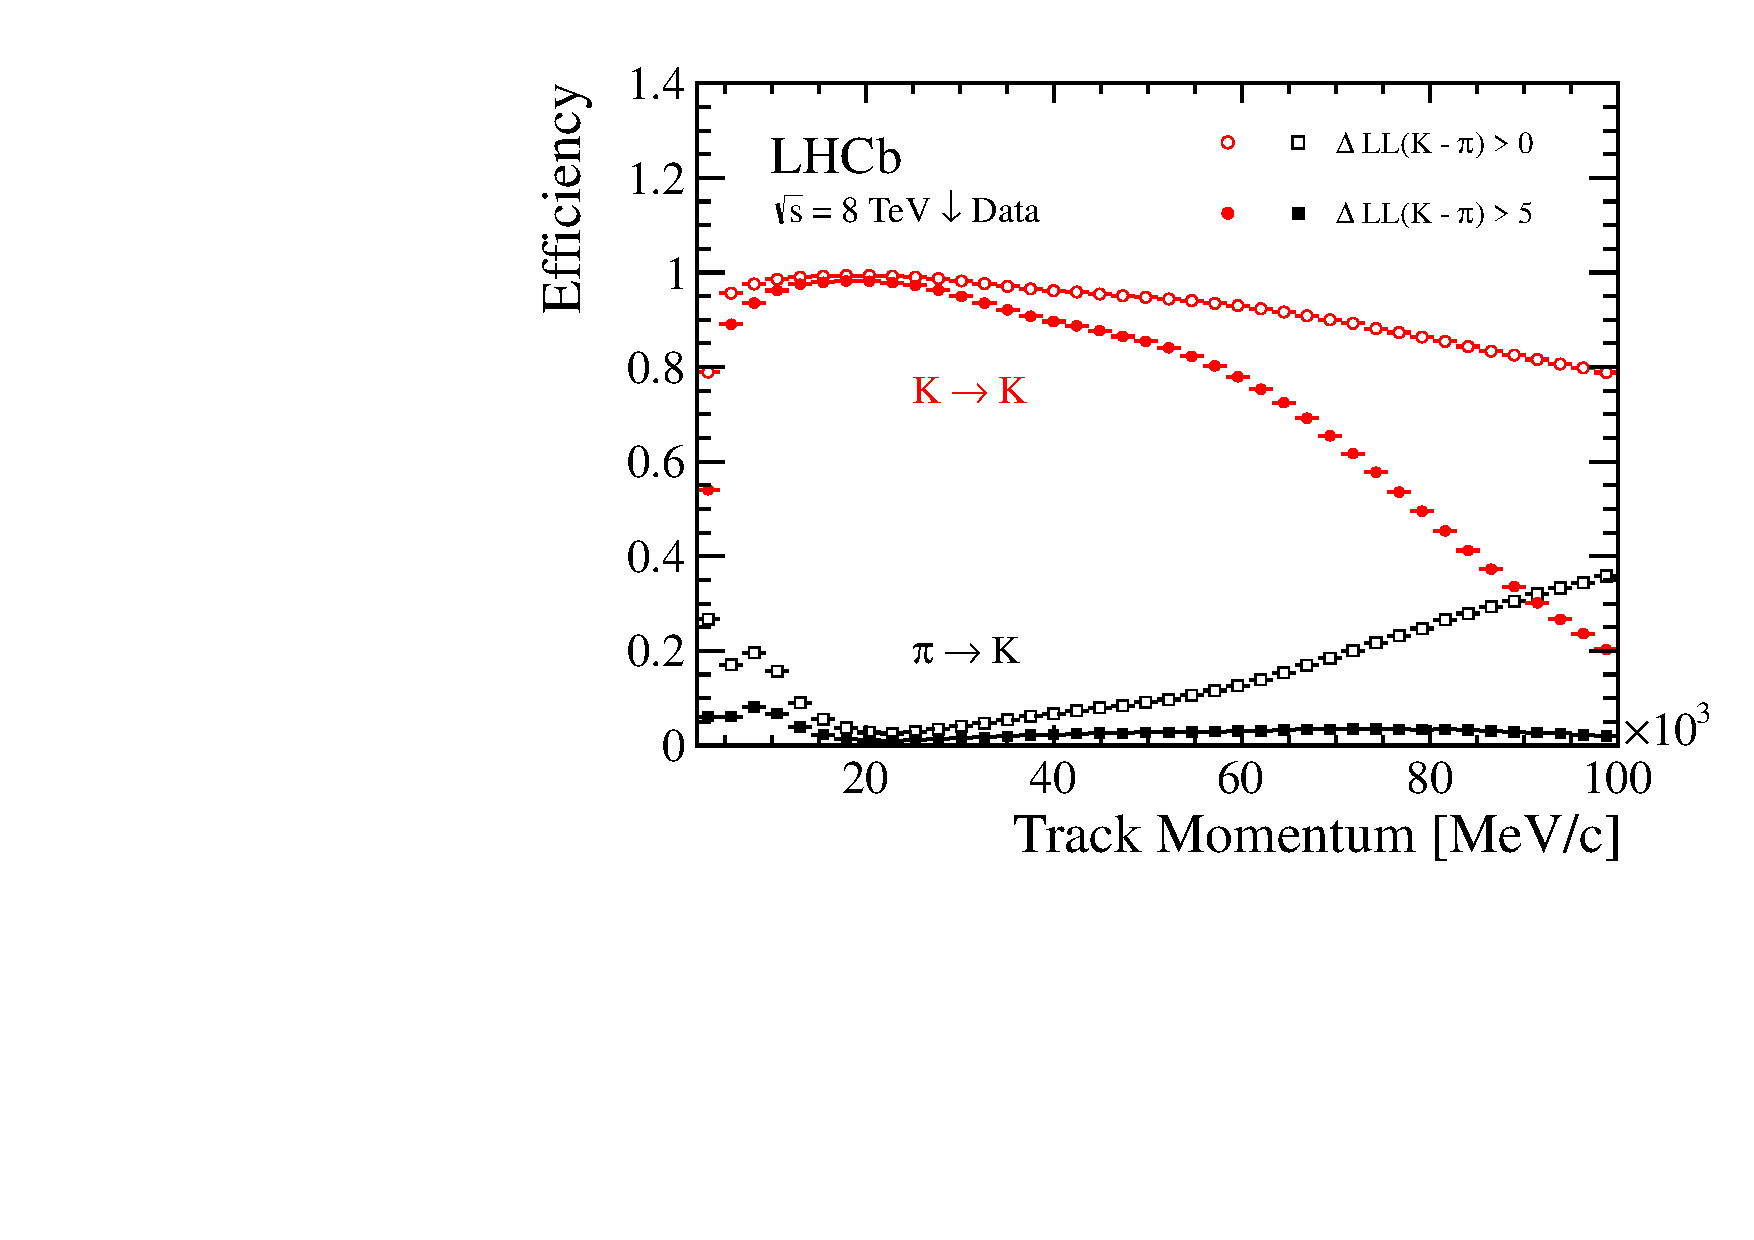
\includegraphics[height=0.2\textheight]{KPi_S20_MagDown_DLL}
  %\end{center}
  %\caption[Particle identification and Cherenkov angles]
  %{\small
    %Cherenkov angle as a function of momentum for pions, kaons and protons in the three different
    %radiators (left), and the kaons-pion separation performance as a function of momentum, from
    %Ref.~\cite{LHCb-DP-2012-003}.
  %}
  %\label{fig:lhcb:pideff}
%\end{figure}

%The detector systems downstream of \richtwo, namely the muon and calorimetry systems, are used for
%\pid and in the trigger; triggering will be covered in the following section.
%As discussed, the \rich detectors excel in hadron identification; for the identification of
%electrons, photons and muons information from the five muon stations (M1-5) and calorimetry system
%are used.
%The calorimeters are situated between M1 and M2-5.

%The general structure of the calorimetry system is that of an \ecal followed by an \hcal.
%The \ecal is a shashlik detector, made of alternating layers of lead, reflector and scintillating
%material, and the light is read out by photomultipliers.
%This subdetector is 25 radiation lengths long to ensure that all electromagnetic energy is
%deposited within before the \hcal.
%It has an energy resolution of $\sigma_E/E = 10\%/\sqrt{E} \oplus 1\%$ where $E$ is in GeV.
%Two additional subdetectors, the \spd and \presh, provide some particle identification at trigger
%level, details of the trigger are provided later.
%Showers caused by the interaction of electromagnetic particles interacting with a thin lead plate
%are detected in the \presh.
%Further upstream of the layer of lead is the \spd, which identifies charged tracks.
%The \hcal consists of layers of iron and scintillating tiles which run parallel to oncoming
%particles.
%Each subdetector within the calorimetry system has increased cell density near the beam to cope
%with higher track multiplicity in this region
%Due to restrictions in space, the \hcal is only 5.6 nuclear interaction lengths long, and has a
%resolution of $\sigma_E/E = (69\pm5)\%/\sqrt{E} \oplus (9\pm2)\%$, where $E$ is in GeV.


%Finally, there is the muon system.
%Each station uses Multi-Wire Projection Chambers exclusively, except for the centre of M1, where
%the expected flux would age this technology too quickly; in this area Gas Electron Multiplier
%detectors are used.
%Like the calorimeters, the muon stations have increased cell density near the beam; however in
%contrast, the cell density is greater in the bending plane than the non-bending plane in order to
%increase momentum resolution.
%Only muon stations M2-5 are used for particle identification; theses are interleaved with plates of
%$80\cm$ thick lead plates, so only very energetic muons reach M5.
%For this reason M4 and M5 are used to identify these penetrating muons, while M2 and M3 have
%increased single hit resolution for momentum measurements.
%In many \lhcb analyses a muon is identified based on hits within the muon system, the criteria is
%known as {\tt isMuon}.
%It is defined as follows: particles with momenta $3<p<6\gev$ must be associated with hits in M2 and M3; if
%$6<p<10\gev$ there must be hits in M2, M3 and either M4 or M5; else if $p>10\gev$ there must be
%associated hits in all M2-5.


